% =============================================================================
%  IV-2-9 — Бие даалт 1 гарын авлага
%  F.CSM302 Үйлдлийн систем, Бие даалт 1.  Хөрвүүлэгч: XeLaTeX (Overleaf: Menu → Compiler)
%  Энэ файлыг tools/build_docs.py бодит тест, туршилтын үр дүнгээс үүсгэсэн; шууд засаж болно.
% =============================================================================
\documentclass[12pt,a4paper]{article}
\usepackage{shutis}

% ---------------- Баримтын мэдээлэл (энд засна) ----------------
\newcommand{\DocTopic}{"Designing a Thread Pool. Programming Project 1 (7-р бүлэг), Worker activity"}
\newcommand{\DocCode}{IV-2-9}
\newcommand{\DocTeacher}{Г.Ганбат /F.CS10/}
\newcommand{\DocCity}{Улаанбаатар хот}
\newcommand{\DocYear}{2026 он}
\newcommand{\DocTeam}{%   \member{Овог.Нэр}{Оюутны код}
  \member{Ц.Номинжин}{B241940137}
  \member{Е.Айсауле}{B221940407}
  \member{Б.Балжинням}{B231940033}
  \member{М.Бат-Орших}{B200930061}
  \member{Г.Хулан}{B241940027}
  \member{Э.Энхсайхан}{B242270097}
}
\hypersetup{pdftitle={IV-2-9 — Бие даалт 1 гарын авлага}, pdfauthor={F.CSM302 IV-2-9 баг}}

\begin{document}
\makecover{ГАРЫН АВЛАГА}

\tableofcontents
\clearpage

% ======================================================================
\section{Хэрэглэгчийн заавар}

\subsection{Программын зорилго}

Сурах бичгийн 7-р бүлгийн thread pool-ийг C хэл дээр pthreads, mutex, POSIX semaphore-оор хэрэгжүүлсэн. Client thread task-уудыг queue-д хийж, worker thread-үүд нь queue-ээс авч гүйцэтгэнэ. Browser дээрх дэлгэц нь \textbf{бодит C программын} үйлдлийг (submit, татгалзал, эхлэх, дуусах, shutdown) worker бүрийн төлөв, queue болон timeline хэлбэрээр харуулна. Дэлгэц зөвхөн харуулдаг; бүх синхрончлол C core дотор явагдана.

\subsection{Дэмжих орчин}

\begin{itemize}
  \item Linux (Ubuntu 22.04+, Debian, Fedora), macOS (Apple Silicon / Intel), Windows дээр \textbf{WSL2 Ubuntu} дотор.
  \item Browser: Chrome, Edge, Firefox, Safari-ийн сүүлийн хувилбар.
  \item Windows дээр шууд ажиллахгүй (pthreads, POSIX semaphore ашигладаг): \textbf{WSL2} эсвэл \textbf{virtual machine} доторх Ubuntu ашиглана.
\end{itemize}

\subsection{Windows: WSL2}

\begin{enumerate}
  \item PowerShell-ийг администратороор нээж \code{wsl --install -d Ubuntu}, компьютераа дахин асаана.
  \item Ubuntu терминалд compiler, Python суулгана:
\end{enumerate}

\par\noindent\begin{minipage}{\linewidth}\setlength{\topsep}{1pt}\setlength{\partopsep}{0pt}
\begin{Verbatim}[commandchars=\\\{\}]
sudo\PY{+w}{ }apt\PY{+w}{ }update\PY{+w}{ }\PY{o}{\PYZam{}\PYZam{}}\PY{+w}{ }sudo\PY{+w}{ }apt\PY{+w}{ }install\PY{+w}{ }\PYZhy{}y\PY{+w}{ }build\PYZhy{}essential\PY{+w}{ }git\PY{+w}{ }python3
\end{Verbatim}
\end{minipage}

\begin{enumerate}
  \item "Суулгах, нээх" хэсгийн командуудыг Ubuntu дотор ажиллуулна. Windows-ийн browser дээр http://localhost:8000 шууд нээгдэнэ.
\end{enumerate}

\subsection{Windows: virtual machine}

VirtualBox, VMware эсвэл UTM дээр Ubuntu 22.04+ суулгаж, WSL2-ийн 2-р алхмын адил \code{build-essential}, \code{python3} суулгана.

\begin{itemize}
  \item VM доторх browser-оос: \code{make ui}, http://localhost:8000.
  \item Windows (host) browser-оос: сервер анхдагчаар зөвхөн VM дотроос хүсэлт хүлээн авдаг тул \code{python3 tools/server.py --host 0.0.0.0} гэж ажиллуулаад \code{http://<VM-ийн IP>:8000} нээнэ (IP-г \code{hostname -I}-ээр харна).
  \item VM-ийн сүлжээ Bridged эсвэл Host-only байна; NAT бол 8000 портыг forward хийнэ.
\end{itemize}

\subsection{Суулгах, нээх}

\par\noindent\begin{minipage}{\linewidth}\setlength{\topsep}{1pt}\setlength{\partopsep}{0pt}
\begin{Verbatim}[commandchars=\\\{\}]
git\PY{+w}{ }clone\PY{+w}{ }https://github.com/NominjinNomio/F.CSM302\PYZhy{}BD\PYZus{}IV\PYZhy{}2\PYZhy{}9\PYZhy{}threadpool.git
\PY{n+nb}{cd}\PY{+w}{ }F.CSM302\PYZhy{}BD\PYZus{}IV\PYZhy{}2\PYZhy{}9\PYZhy{}threadpool
make\PY{+w}{          }\PY{c+c1}{\PYZsh{} C программыг build хийнэ}
make\PY{+w}{ }ui\PY{+w}{       }\PY{c+c1}{\PYZsh{} http://localhost:8000}
\end{Verbatim}
\end{minipage}

Дараа нь browser-т \textbf{http://localhost:8000}-ийг нээнэ. Баруун дээд буланд ногоон цэг ба "C программтай холбогдсон" гэж гарвал бэлэн. Хуудас нээгдэхэд анхдагч тохиргоогоор нэг удаа автоматаар ажиллана.

\subsection{Дэлгэцийн бүтэц}

Дэлгэц зүүн талын тохиргоо, баруун талын дүрслэлээс бүрдэнэ (Хүснэгт \ref{tab:regions}, Зураг \ref{fig:overview}).

\begin{table}[H]
\centering
\caption{Дэлгэцийн хэсгүүд}\label{tab:regions}
\begin{tabular}{|P{0.280}|P{0.180}|P{0.540}|}
\hline
\rowcolor{tablehead} \textbf{Хэсэг} & \textbf{Байрлал} & \textbf{Юу хийх вэ} \\ \hline
Pool тохиргоо & зүүн дээд & worker, queue, дүүрэх үеийн бодлого, retry зай \\ \hline
Ачаалал (task) & зүүн доод & Параметрээр эсвэл Task жагсаалтаар task үүсгэх; Ажиллуулах, Анхдагч, Trace ачаалах/хадгалах \\ \hline
Playback мөр & баруун дээд & Reset, өмнөх/дараагийн үйлдэл, тоглуулах, хугацааны гулсуур, хурд \\ \hline
Worker-ууд, Task queue & дунд & t агшин дахь worker бүрийн төлөв, queue-ийн нүд, тоолуур, үйлдлийн тайлбар \\ \hline
Worker activity timeline & дунд & worker бүрийн хугацааны мөр, client мөр, queue-ийн урт \\ \hline
Үр дүн ба шалгалт & доор & хэмжүүрүүд, 8 шалгалт, C программын команд ба гаралт \\ \hline
Үйлдлийн бүртгэл & хамгийн доор & үйлдэл бүрийн хүснэгт; мөр дээр дарж тэр агшин руу очно \\ \hline
\end{tabular}
\end{table}

\begin{figure}[H]
\centering
{\setlength{\fboxsep}{0pt}\setlength{\fboxrule}{0.5pt}\fcolorbox{frameline}{white}{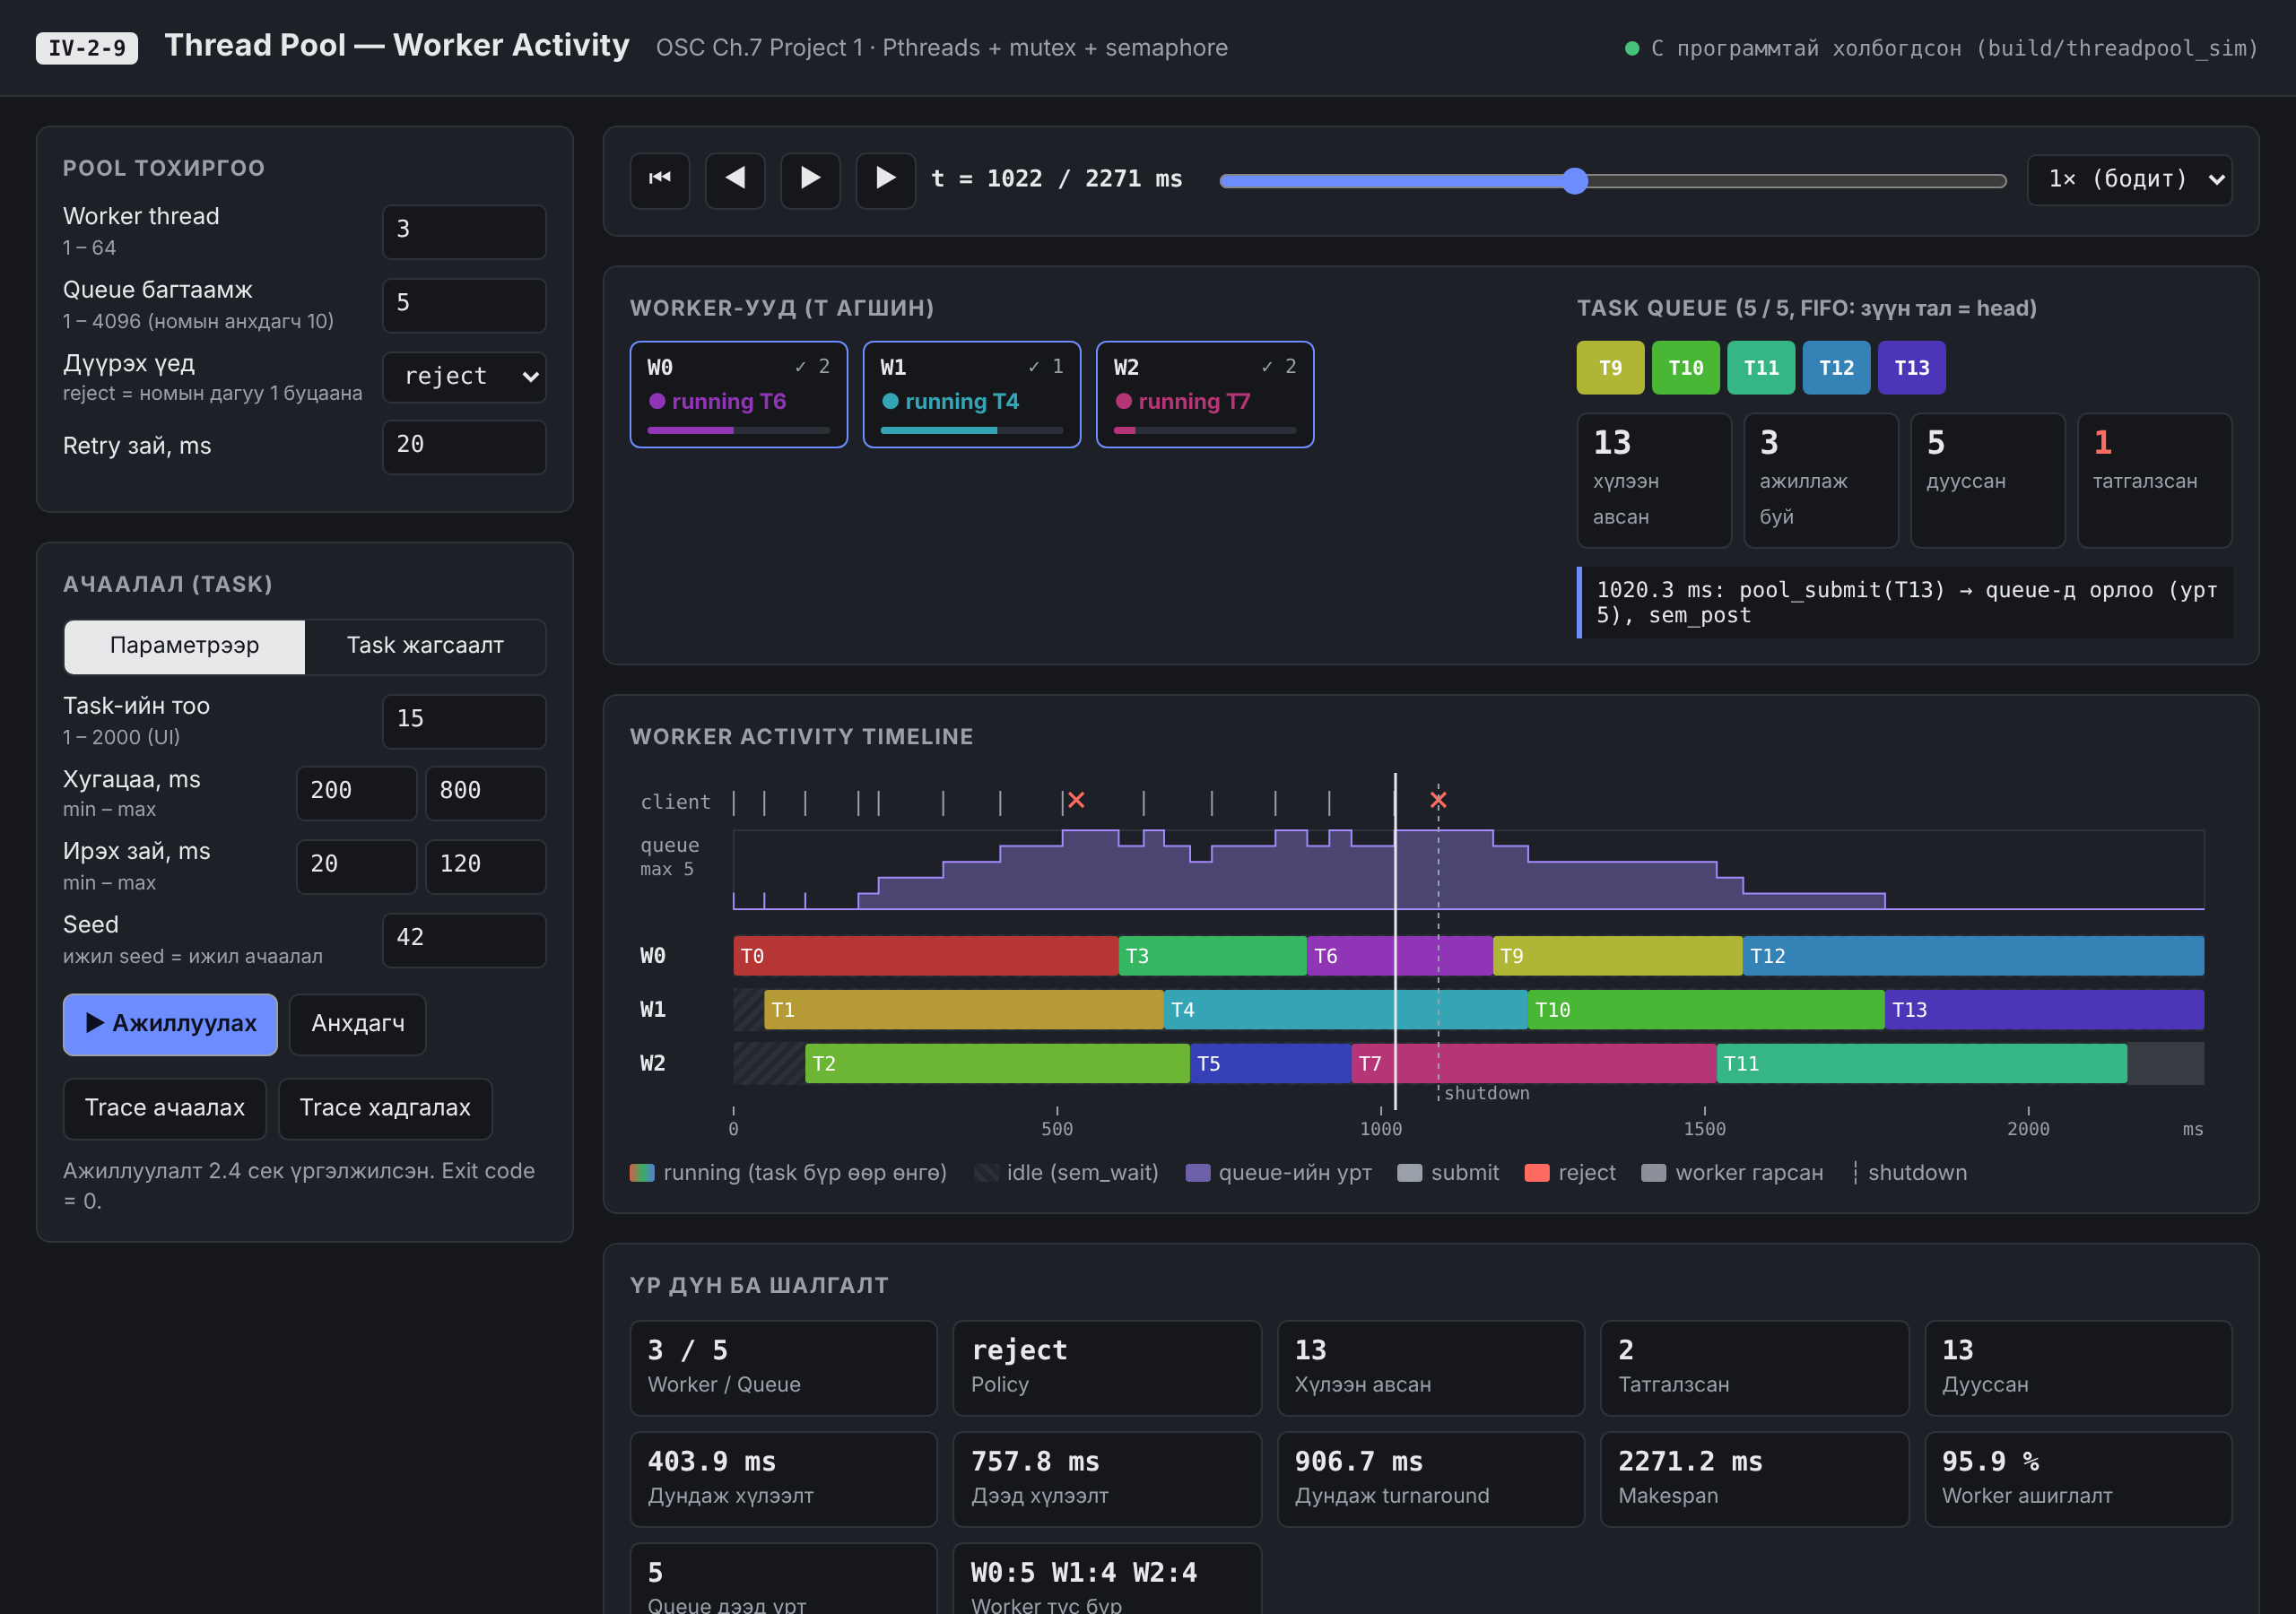
\includegraphics[width=0.88\linewidth]{img/shots/overview.png}}}
\caption{Дэлгэцийн ерөнхий харагдац}\label{fig:overview}
\end{figure}

\subsection{Оролт ба тохиргоо}

Тоо бүрийг шууд бичиж эсвэл сумаар өөрчилнө. Хүрээнээс гадуур утга оруулбал Ажиллуулах дарахад улаан талбарт алдааны тайлбар гарна (Зураг \ref{fig:err}). \textbf{Параметрээр} горимд task-уудыг seed-ээс санамсаргүй үүсгэнэ; \textbf{Task жагсаалт} горимд мөр бүрт \code{arrival\_ms duration\_ms} бичнэ (\code{\#}-ээс хойш тайлбар, arrival өсөх дарааллаар). \textbf{Бэлэн тест}-ээс \code{basic.txt}, \code{burst.txt}, \code{fifo.txt}, \code{mixed\_long\_short.txt} сонгож болно.

\begin{longtable}{|P{0.220}|P{0.460}|P{0.170}|P{0.150}|}
\caption{Оролт ба тохиргоо}\label{tab:input}\\
\hline
\rowcolor{tablehead} \textbf{Талбар} & \textbf{Утга} & \textbf{Хүрээ} & \textbf{Анхдагч} \\ \hline
\endfirsthead
\hline
\rowcolor{tablehead} \textbf{Талбар} & \textbf{Утга} & \textbf{Хүрээ} & \textbf{Анхдагч} \\ \hline
\endhead
Worker thread & pool дахь worker thread-ийн тоо & 1-64 & 3 \\ \hline
Queue багтаамж & тойрог массив queue-ийн хэмжээ & 1-4096 & 5 \\ \hline
Дүүрэх үед & reject: \code{pool\_submit} 1 буцааж task хаягдана; retry: client хүлээгээд дахин оролдоно & reject / retry & reject \\ \hline
Retry зай (мс) & retry горимд дахин оролдох зай & 1-10000 & 20 \\ \hline
Task-ийн тоо & үүсгэх task-ийн тоо & 1-2000 & 15 \\ \hline
Хугацаа (мс) & task бүрийн хугацаа энэ мужаас санамсаргүй & 1-60000 & 200-800 \\ \hline
Ирэх зай (мс) & дараалсан task-уудын зай; 0 = бүгд зэрэг & 0-60000 & 20-120 \\ \hline
Seed & ижил seed = ижил ачаалал & ≥ 0 & 42 \\ \hline
\end{longtable}

\begin{figure}[H]
\centering
{\setlength{\fboxsep}{0pt}\setlength{\fboxrule}{0.5pt}\fcolorbox{frameline}{white}{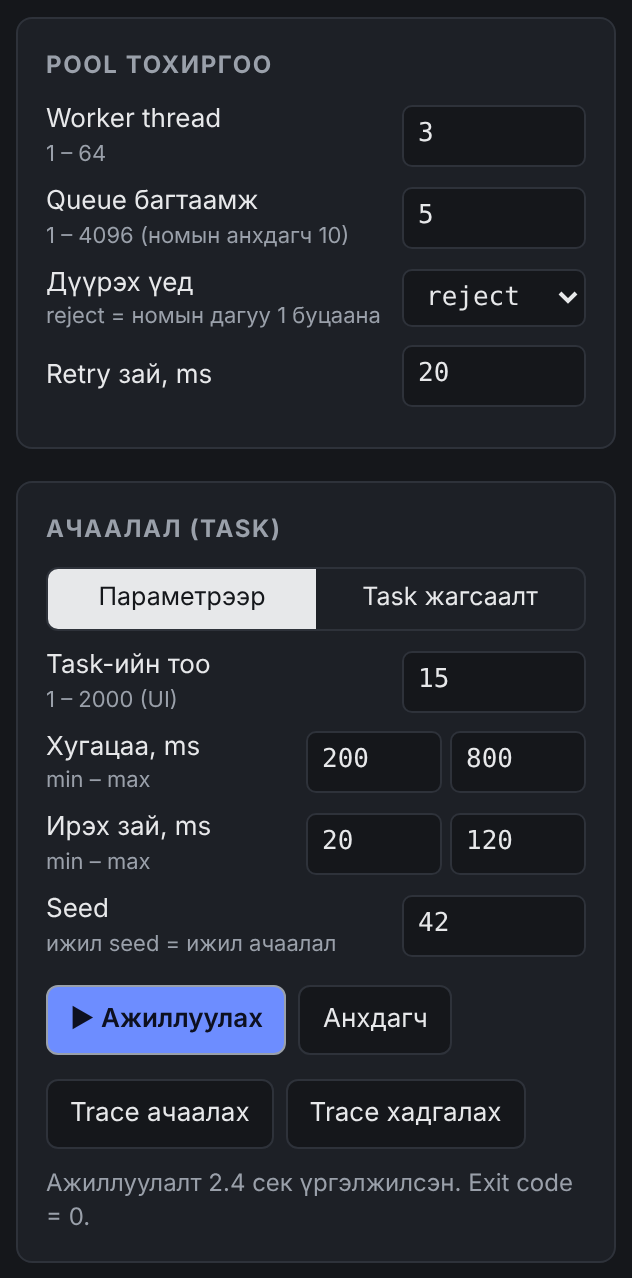
\includegraphics[width=0.38\linewidth]{img/shots/settings.png}}}
\caption{Тохиргоо}\label{fig:settings}
\end{figure}

\subsection{Ажиллуулах, зогсоох, reset}

\begin{itemize}
  \item \textbf{Ажиллуулах}: тохиргоогоор C программыг бодитоор ажиллуулна (task-уудын нийт хугацаа шиг үргэлжилнэ), дараа нь автоматаар тоглуулна.
  \item \textbf{▶ / ‖} (\kbd{Space}): тоглуулах, түр зогсоох. \textbf{◀ / ▶} (\kbd{←} \kbd{→}): өмнөх, дараагийн үйлдэл рүү алхах.
  \item \textbf{Гулсуур}, timeline дээр \textbf{дарах эсвэл чирэх}, бүртгэлийн мөр дээр дарах: тухайн агшин руу очно.
  \item \textbf{Хурд}: 0.25×, 0.5×, 1× (бодит хугацаа), 2×, 4×, 10×.
  \item \textbf{|◀ Reset}: эхний агшин руу буцна. \textbf{Анхдагч}: бүх тохиргоог анхны утганд оруулна.
  \item \textbf{Trace хадгалах}: тухайн ажиллалтыг JSON файлаар татна. \textbf{Trace ачаалах}: хадгалсан trace-ийг дахин нээнэ.
  \item \textbf{Серверийг зогсоох}: терминалд \kbd{Ctrl}+\kbd{C}.
\end{itemize}

\subsection{Дүрслэлийн тэмдэг, өнгө, төлөв}

\textbf{Worker карт.} Worker бүр нэг карт: нэр (W0, W1…), одоогийн төлөв, явцын шугам, баруун дээд буланд дуусгасан task-ийн тоо (✓ n).

\begin{itemize}
  \item \textbf{● running Tk} (өнгөт, хүрээ цэнхэр): worker Tk task-ийг гүйцэтгэж байна (\textit{running}).
  \item \textbf{○ idle — sem\_wait} (саарал): worker semaphore дээр ажил хүлээж байна (\textit{idle}).
  \item \textbf{■ exited} (бүдэг): shutdown-ы дараа worker гарсан. ✓ n нь тухайн worker-ийн \textit{completed} task-ийн тоо.
\end{itemize}

\textbf{Task queue.} Хүлээж буй task-ууд өөрийн өнгөөр, зүүн талд нь хамгийн түрүүнд авагдах (head). Тасархай хүрээтэй нүд = сул зай. Доор нь хүлээн авсан, ажиллаж буй, дууссан, татгалзсан тоо, түүний доор тухайн агшны үйлдлийн тайлбар (жишээ нь "W1 sem\_wait-аас сэрж T10-г dequeue хийв").

\begin{figure}[H]
\centering
{\setlength{\fboxsep}{0pt}\setlength{\fboxrule}{0.5pt}\fcolorbox{frameline}{white}{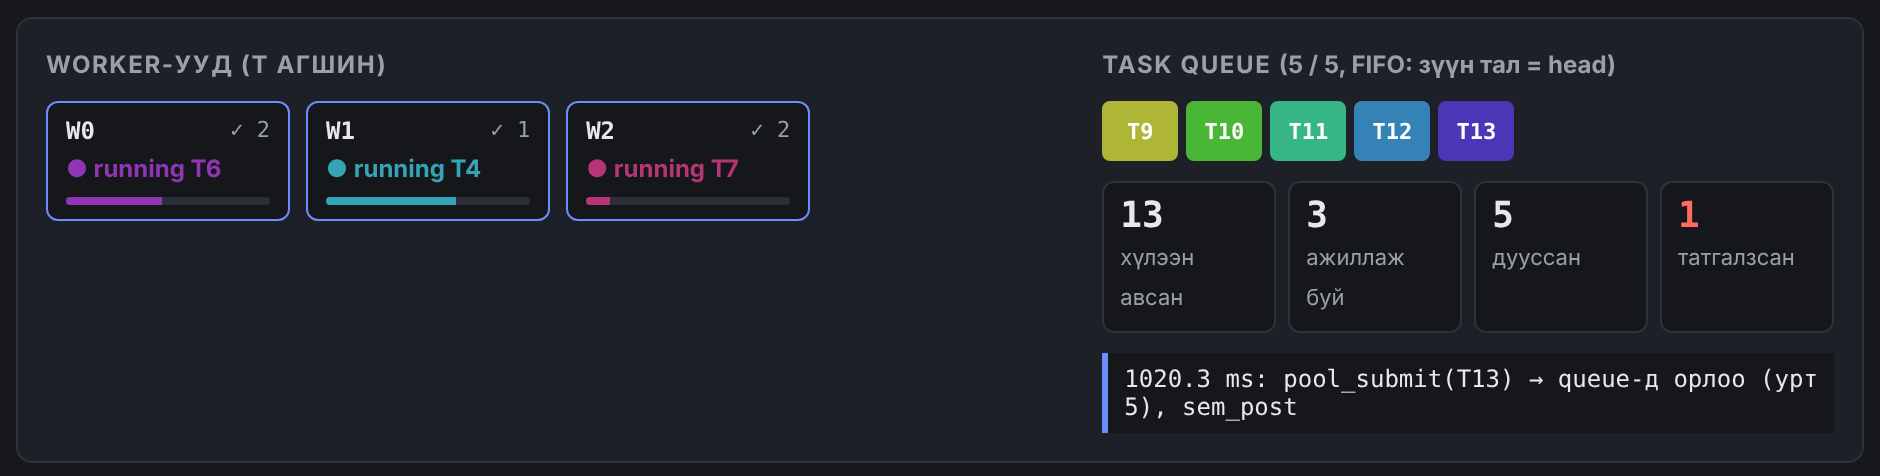
\includegraphics[width=0.85\linewidth]{img/shots/live_state.png}}}
\caption{Worker карт ба task queue}
\end{figure}

\begin{longtable}{|P{0.320}|P{0.680}|}
\caption{Worker activity timeline-ийн тэмдэг}\label{tab:legend}\\
\hline
\rowcolor{tablehead} \textbf{Тэмдэг} & \textbf{Утга} \\ \hline
\endfirsthead
\hline
\rowcolor{tablehead} \textbf{Тэмдэг} & \textbf{Утга} \\ \hline
\endhead
өнгөт зурвас \code{Tk} & worker Tk task-ийг гүйцэтгэсэн хугацаа; task бүр өөр өнгөтэй, queue-д ч мөн тэр өнгөөр харагдана \\ \hline
судалтай саарал & idle: worker \code{sem\_wait} дээр хүлээж байна \\ \hline
бараан бүс & worker гарсан (shutdown-ы дараа) \\ \hline
нил ягаан шатлалт график & queue-ийн урт (0 … багтаамж) \\ \hline
client мөр: саарал | & \code{pool\_submit} амжилттай (0) \\ \hline
client мөр: улаан ✕ & queue дүүрсэн, \code{pool\_submit} 1 буцаасан \\ \hline
тасархай босоо зураас & \code{pool\_shutdown()} дуудагдсан агшин \\ \hline
хар босоо шугам & одоогийн агшин (playhead) \\ \hline
\end{longtable}

\subsection{Жишээ}

\textbf{Жишээ 1. Queue дүүрэх} (Task жагсаалт → burst.txt, W=2, Q=3, reject). 10 task нэгэн зэрэг ирэх тул queue хурдан дүүрнэ: 3-5 task хүлээн авагдаж, үлдсэн нь client мөрөнд улаан ✕ болно. Төгсгөлд \code{VERIFY OK}.

\begin{figure}[H]
\centering
{\setlength{\fboxsep}{0pt}\setlength{\fboxrule}{0.5pt}\fcolorbox{frameline}{white}{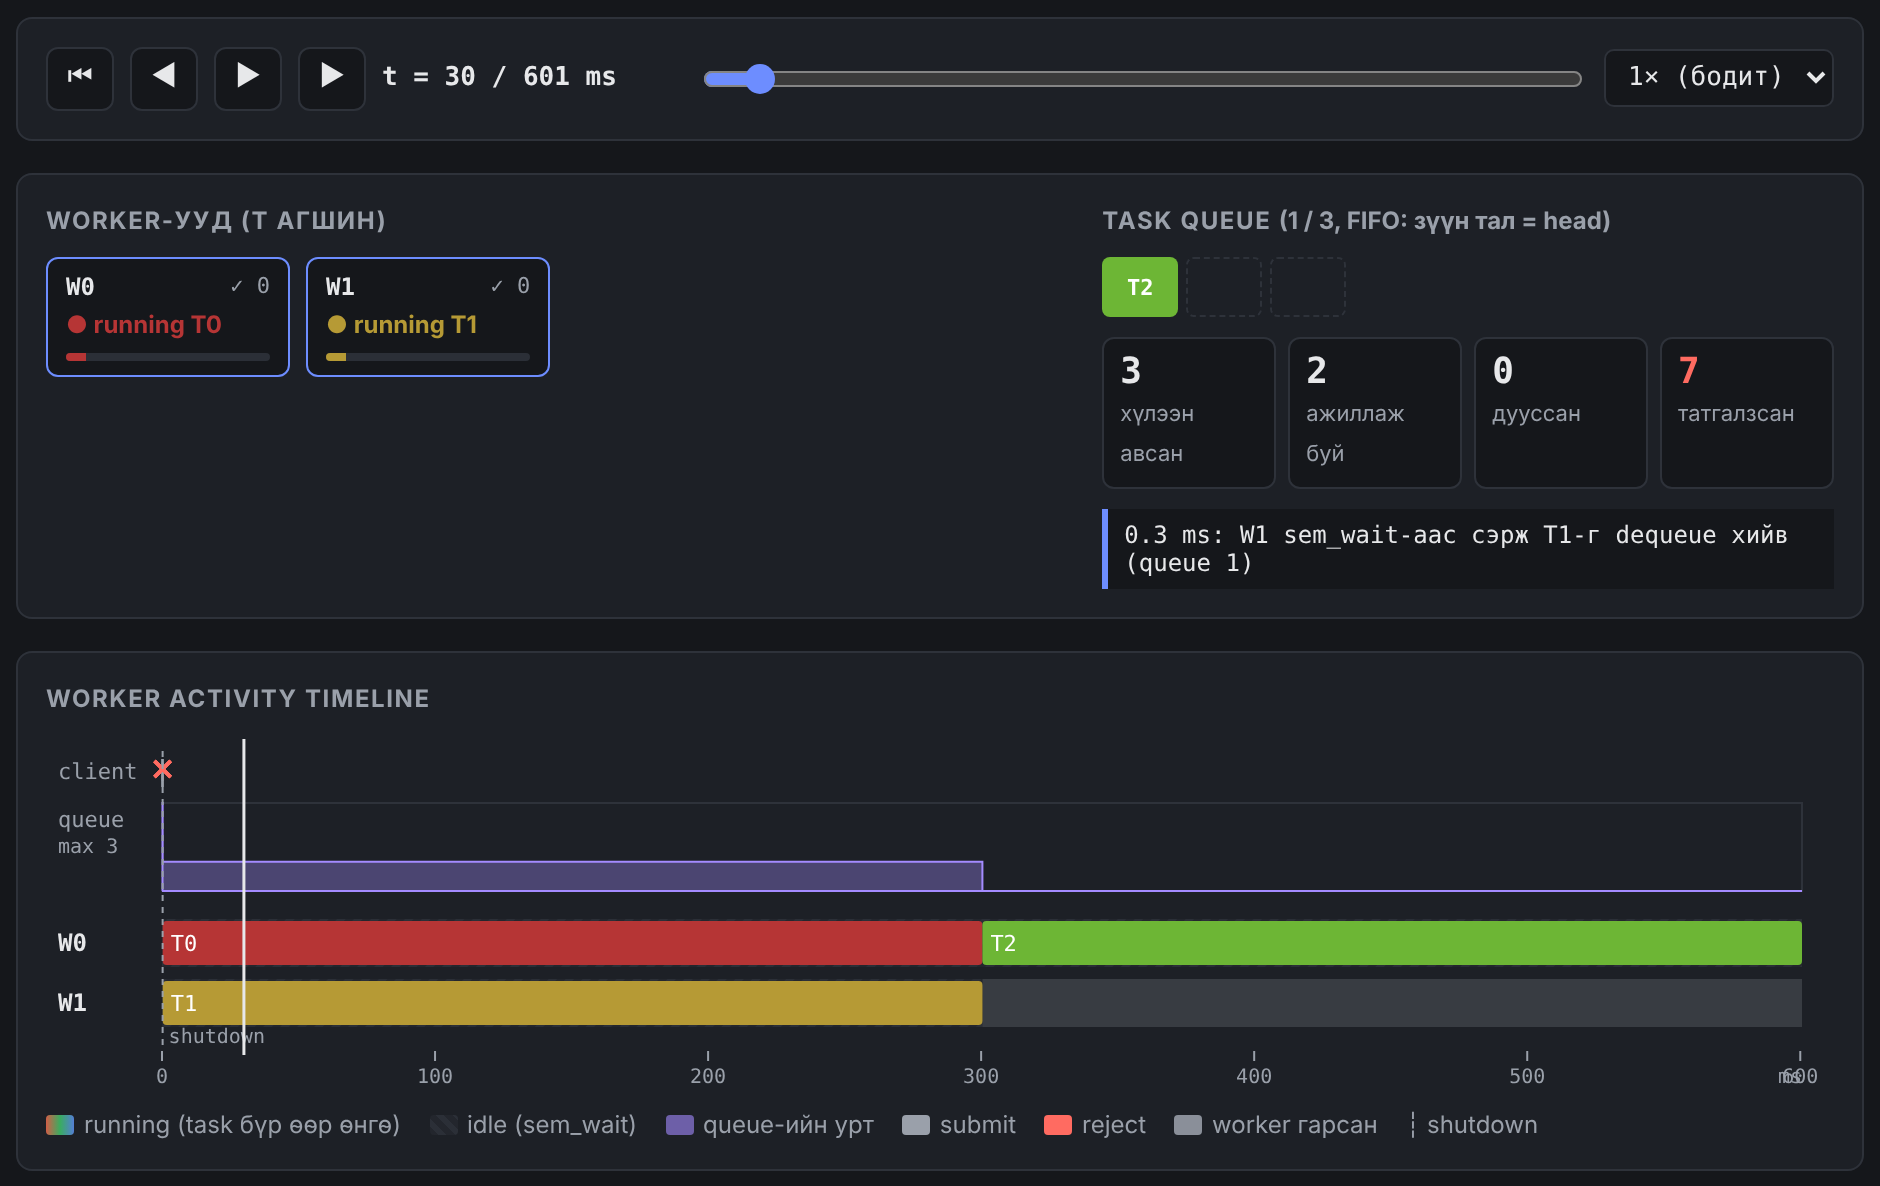
\includegraphics[width=0.72\linewidth]{img/shots/burst_reject.png}}}
\caption{Жишээ 1. Queue дүүрэх}
\end{figure}

\textbf{Жишээ 2. Retry горим} (Жишээ 1-ийн тохиргоо, Дүүрэх үед: retry). Client дүүрсэн queue-д 20 мс тутам дахин оролдох тул ✕ олон боловч 10 task бүгд гүйцэтгэгдэнэ, нийт хугацаа ≈ 1500 мс.

\begin{figure}[H]
\centering
{\setlength{\fboxsep}{0pt}\setlength{\fboxrule}{0.5pt}\fcolorbox{frameline}{white}{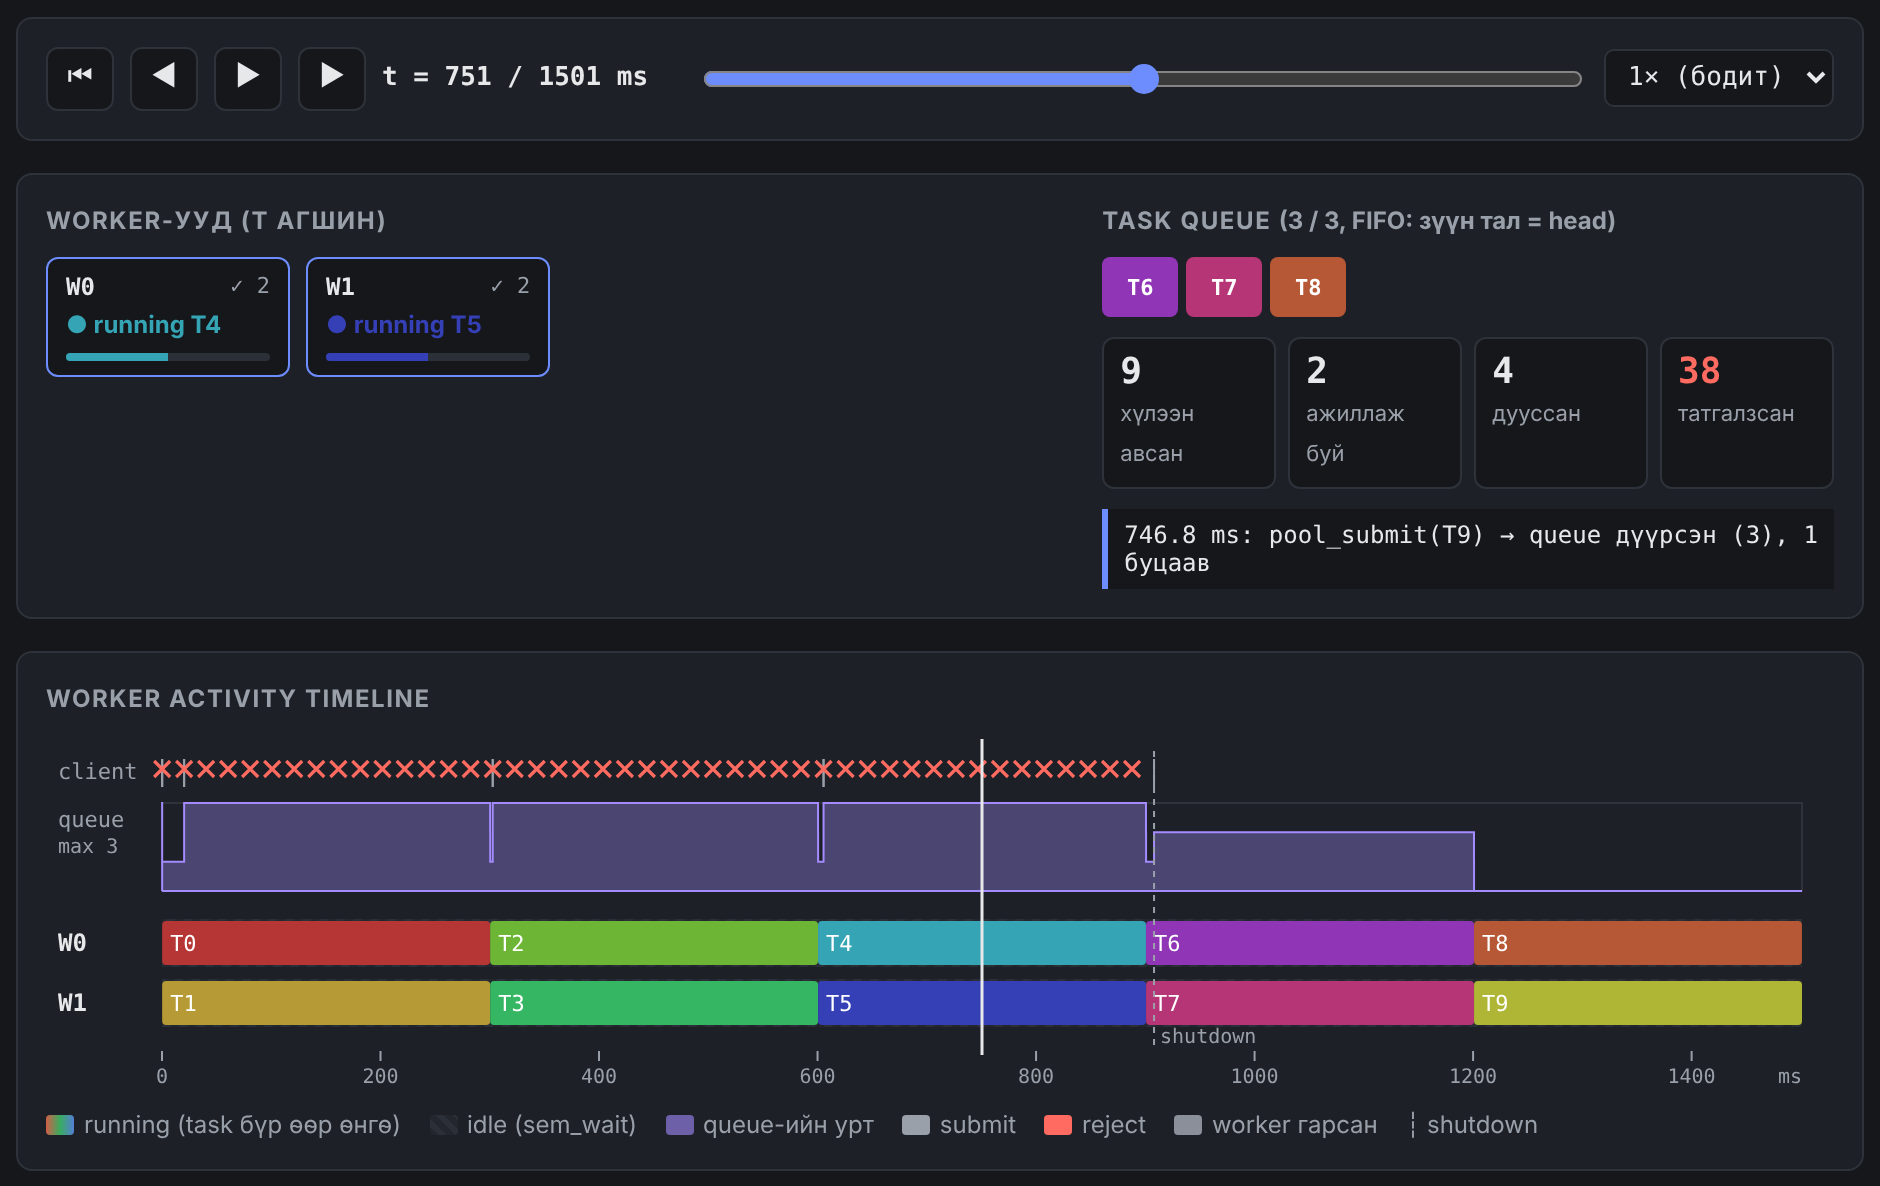
\includegraphics[width=0.72\linewidth]{img/shots/burst_retry.png}}}
\caption{Жишээ 2. Retry горим}
\end{figure}

\textbf{Жишээ 3. FIFO-г алхамчлах} (fifo.txt, W=1, Q=10). Ажиллуулаад |◀ дарж, ▶ (\kbd{→}) товчоор нэг нэгээр алхана. Task-ууд T0, T1, T2… дарааллаар эхэлж, queue-ийн зүүн талаас авагдана.

\begin{figure}[H]
\centering
{\setlength{\fboxsep}{0pt}\setlength{\fboxrule}{0.5pt}\fcolorbox{frameline}{white}{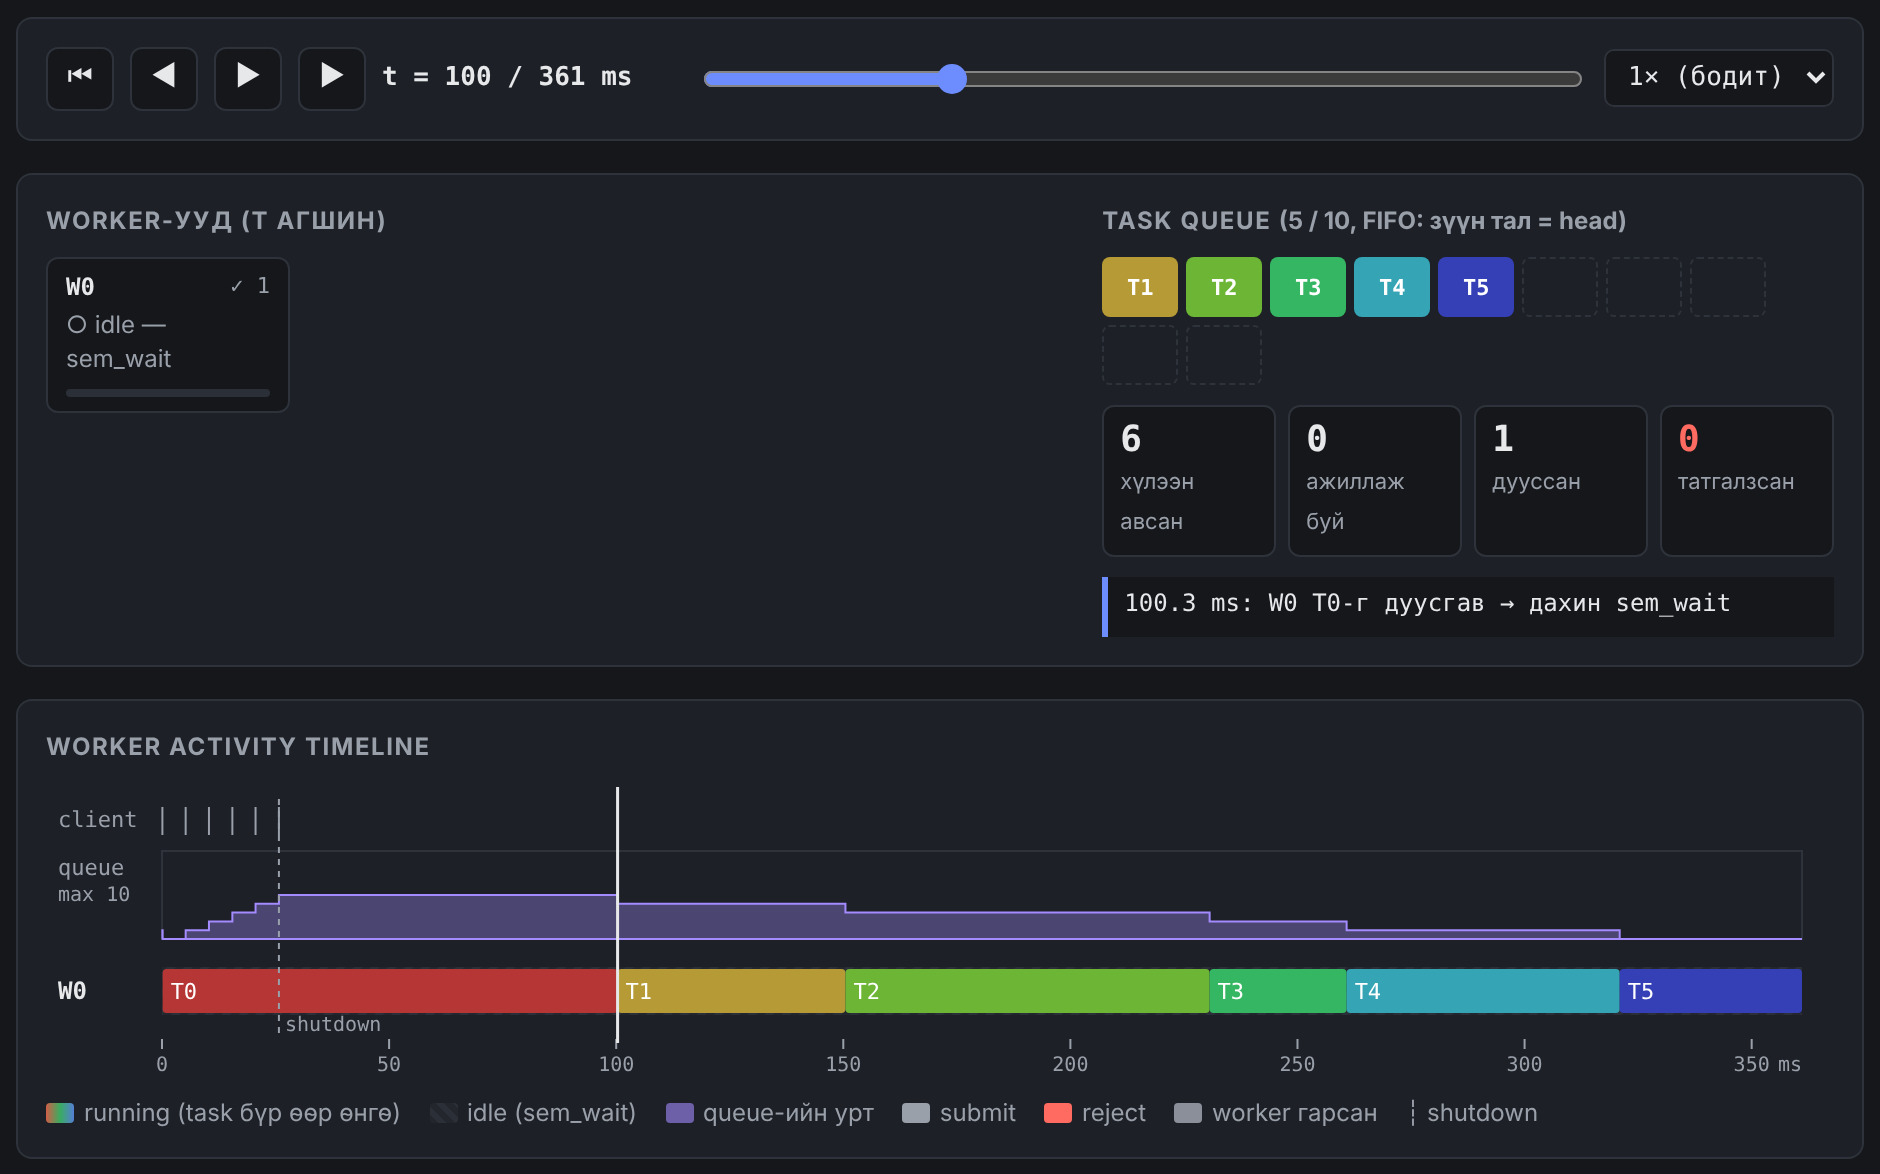
\includegraphics[width=0.72\linewidth]{img/shots/fifo_step.png}}}
\caption{Жишээ 3. FIFO, алхамчилсан}
\end{figure}

\textbf{Жишээ 4. Worker-ийн тооны нөлөө} (Параметрээр: 12 task, хугацаа 100-300, ирэх зай 0-0, queue 64, seed 1). Worker-ийг 1, дараа нь 4 болгож ажиллуулаад timeline болон "Makespan"-ийг харьцуулна.

\begin{figure}[H]
\centering
{\setlength{\fboxsep}{0pt}\setlength{\fboxrule}{0.5pt}\fcolorbox{frameline}{white}{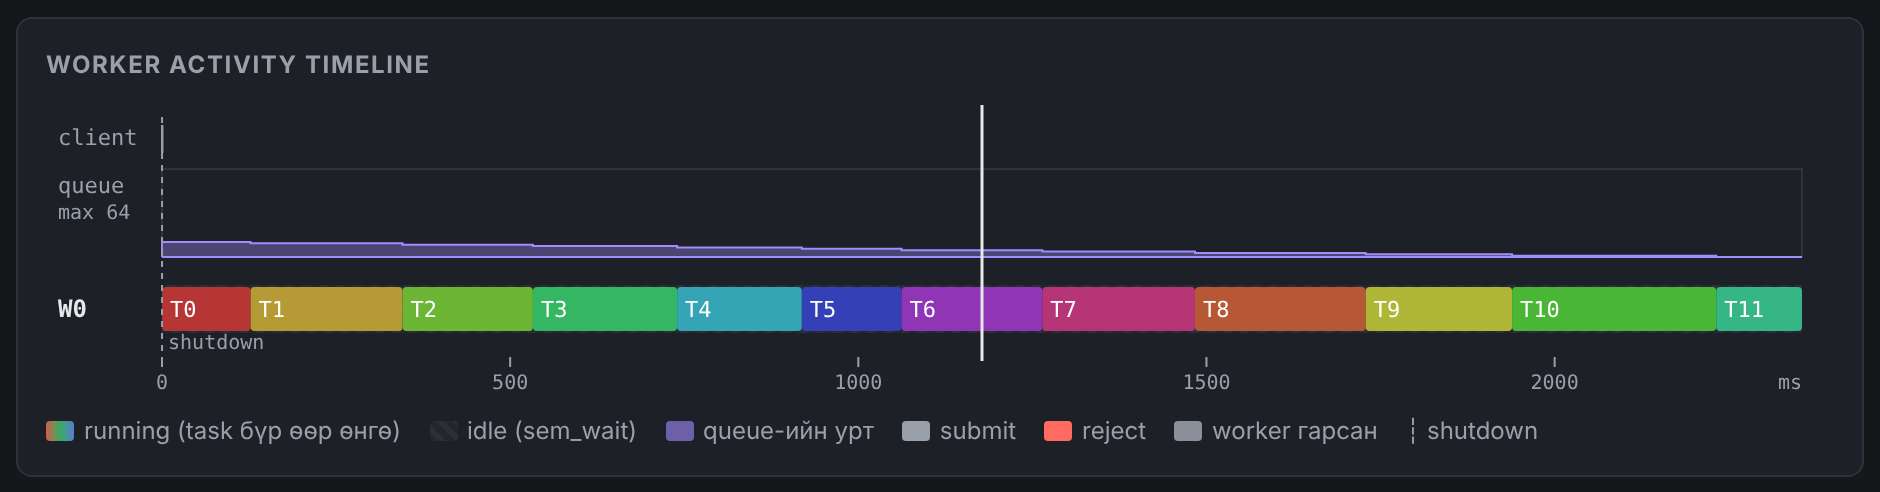
\includegraphics[width=0.78\linewidth]{img/shots/compare_w1.png}}}\\[8pt]
{\setlength{\fboxsep}{0pt}\setlength{\fboxrule}{0.5pt}\fcolorbox{frameline}{white}{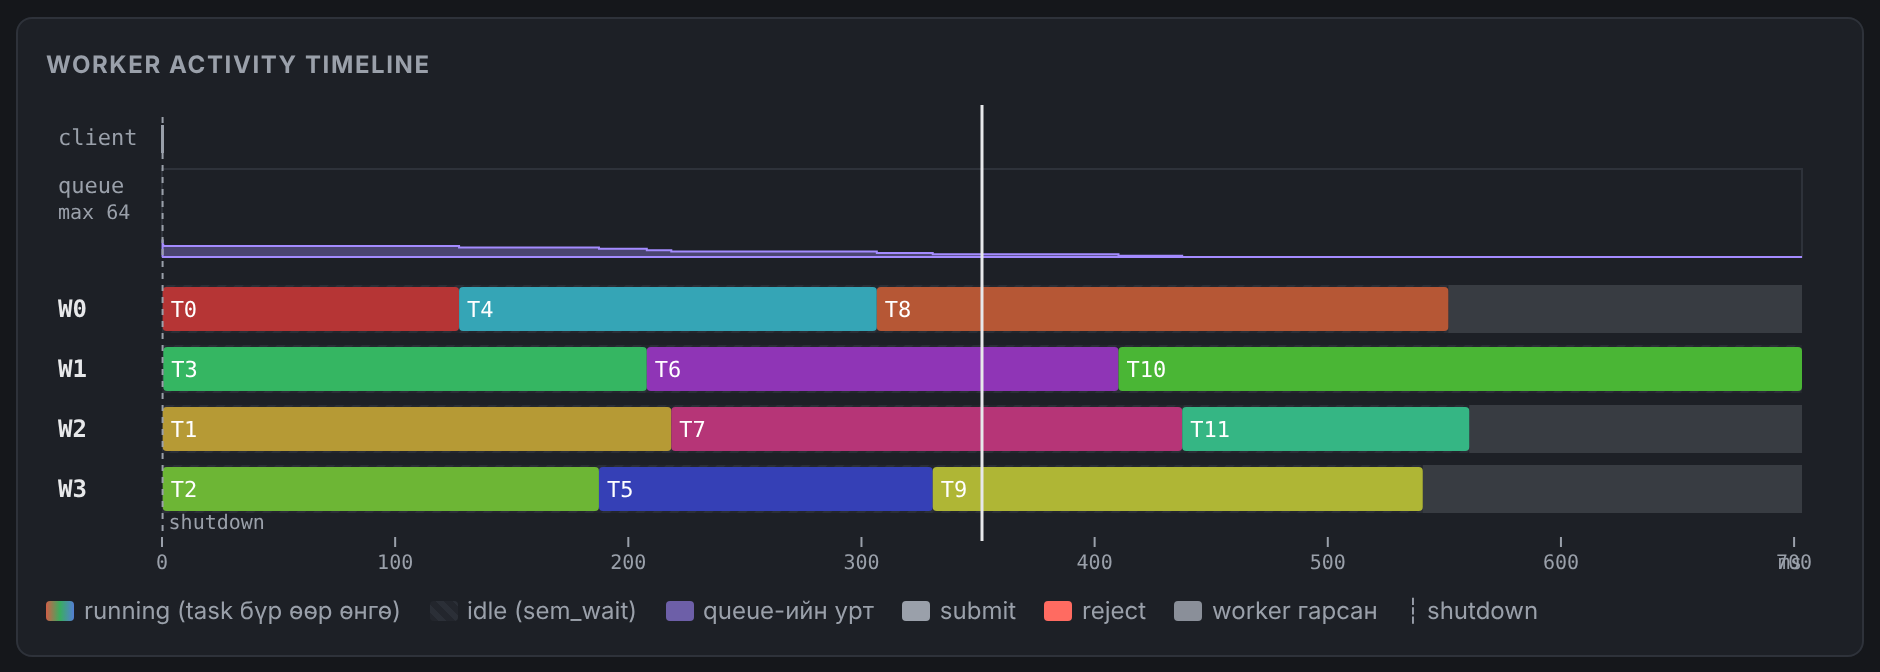
\includegraphics[width=0.78\linewidth]{img/shots/compare_w4.png}}}
\caption{Жишээ 4. Дээр 1 worker, доор 4 worker}
\end{figure}

\textbf{Жишээ 5. Үйлдлийн бүртгэл.} Бүртгэлийн мөр бүр нэг үйлдэл; одоогийн мөр цэнхэрээр, ирээдүйн мөрүүд бүдгээр харагдана. Мөр дээр дарахад тэр агшин руу очно.

\begin{figure}[H]
\centering
{\setlength{\fboxsep}{0pt}\setlength{\fboxrule}{0.5pt}\fcolorbox{frameline}{white}{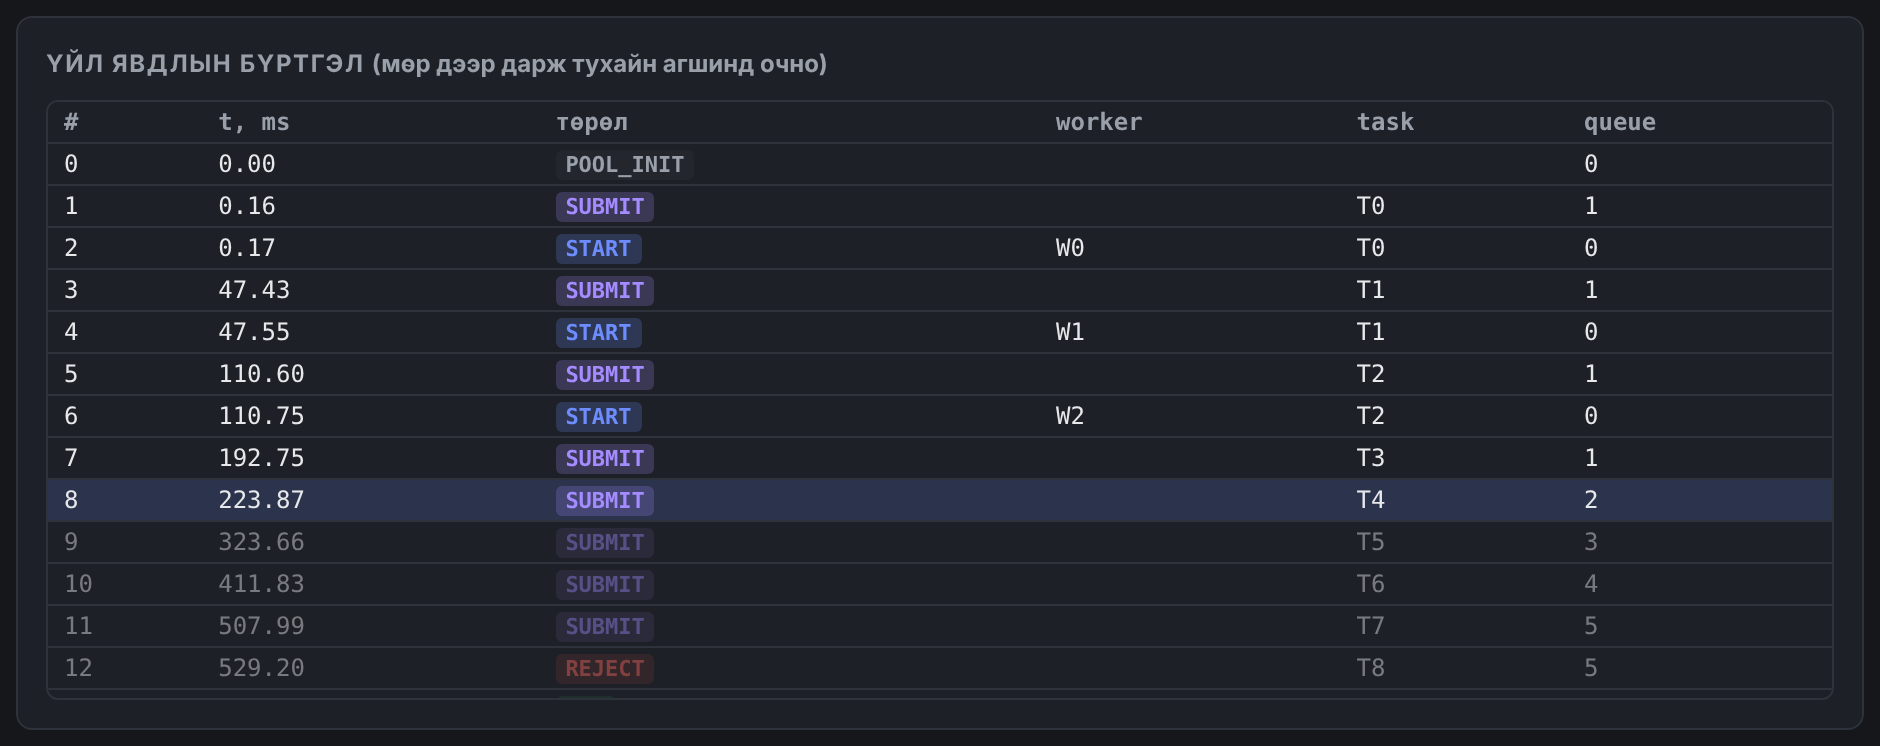
\includegraphics[width=0.72\linewidth]{img/shots/event_log.png}}}
\caption{Жишээ 5. Үйлдлийн бүртгэл}
\end{figure}

\subsection{Сервергүй горим}

\code{ui/index.html}-ийг файлаар шууд нээвэл баруун дээд буланд "offline — зөвхөн trace файл үзэх горим" гарч, Ажиллуулах идэвхгүй болно. \textbf{Trace ачаалах}-аар \code{examples/sample\_trace.json} эсвэл өөрийн хадгалсан trace-ийг нээж бүх дүрслэлийг ашиглаж болно.

\begin{figure}[H]
\centering
{\setlength{\fboxsep}{0pt}\setlength{\fboxrule}{0.5pt}\fcolorbox{frameline}{white}{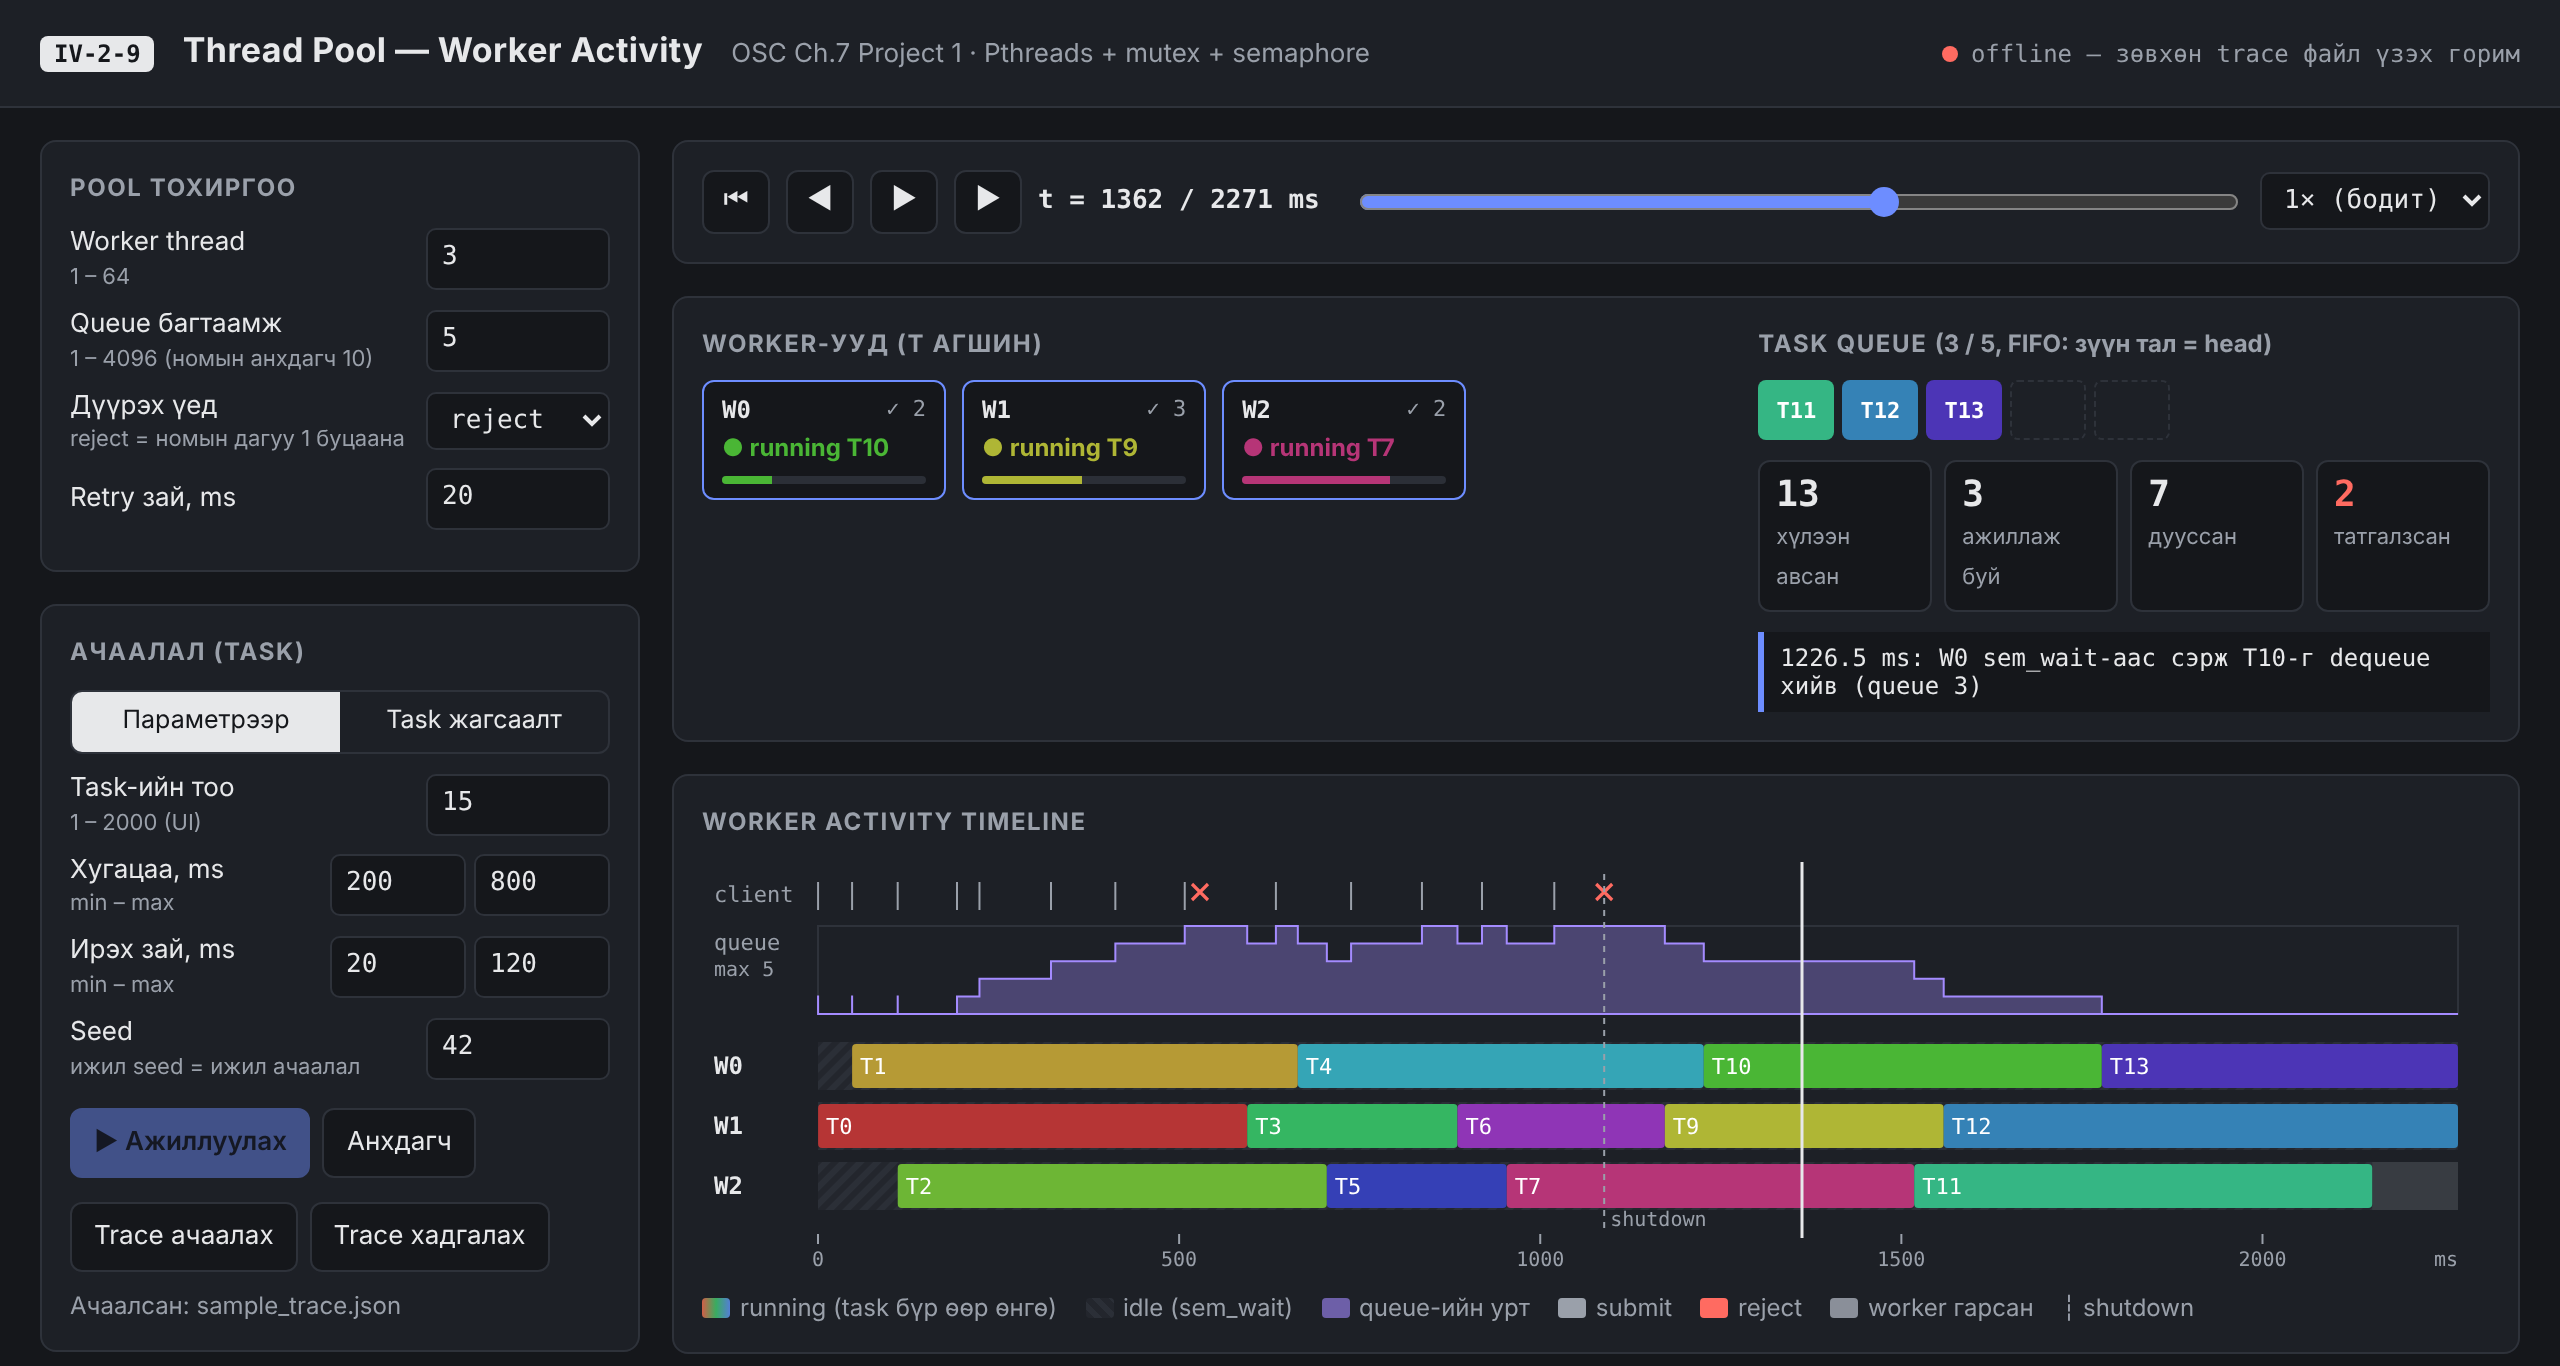
\includegraphics[width=0.82\linewidth]{img/shots/offline.png}}}
\caption{Сервергүй горимд хадгалсан trace үзэж буй нь}
\end{figure}

\subsection{Түгээмэл алдаа ба шийдэл}

\begin{longtable}{|P{0.360}|P{0.280}|P{0.360}|}
\caption{Түгээмэл алдаа}\label{tab:errs}\\
\hline
\rowcolor{tablehead} \textbf{Алдаа} & \textbf{Шалтгаан} & \textbf{Шийдэл} \\ \hline
\endfirsthead
\hline
\rowcolor{tablehead} \textbf{Алдаа} & \textbf{Шалтгаан} & \textbf{Шийдэл} \\ \hline
\endhead
\code{-w буруу ('0'): worker-ийн тоо 1..64} & хүрээнээс гадуур утга & тайлбарт заасан мужид оруулна (Зураг \ref{fig:err}) \\ \hline
\code{<task жагсаалт>:2 — duration\_ms буруу} & жагсаалтын 2-р мөрөнд тоо биш утга & мөр бүр яг 2 бүхэл тоо \\ \hline
\code{arrival\_ms өсөхгүй дарааллаар} & ирэх хугацаа эрэмбэгүй & arrival-аар эрэмбэлнэ \\ \hline
\code{Тооцоолсон хугацаа \textasciitilde{}N сек} & интерфейсийн 60 с-ийн хязгаар & task/хугацааг багасгах, worker нэмэх эсвэл CLI ашиглах \\ \hline
\code{offline — зөвхөн trace} & сервер ажиллаагүй / файлаар нээсэн & \code{make ui}, дараа нь http://localhost:8000 \\ \hline
\code{build/threadpool\_sim алга} & build хийгээгүй & \code{make} \\ \hline
\code{make: cc: No such file} & C compiler байхгүй & Ubuntu/WSL: \code{sudo apt install build-essential}; macOS: \code{xcode-select --install} \\ \hline
\code{Address already in use} & 8000 порт завгүй & \code{python3 tools/server.py --port 8080} \\ \hline
Ижил тохиргоо өөр timeline & OS scheduler-ийн nondeterminism & алдаа биш; Trace хадгалахаар тогтооно \\ \hline
\end{longtable}

\begin{figure}[H]
\centering
\begin{minipage}[t]{0.346\linewidth}\vspace{0pt}{\setlength{\fboxsep}{0pt}\setlength{\fboxrule}{0.5pt}\fcolorbox{frameline}{white}{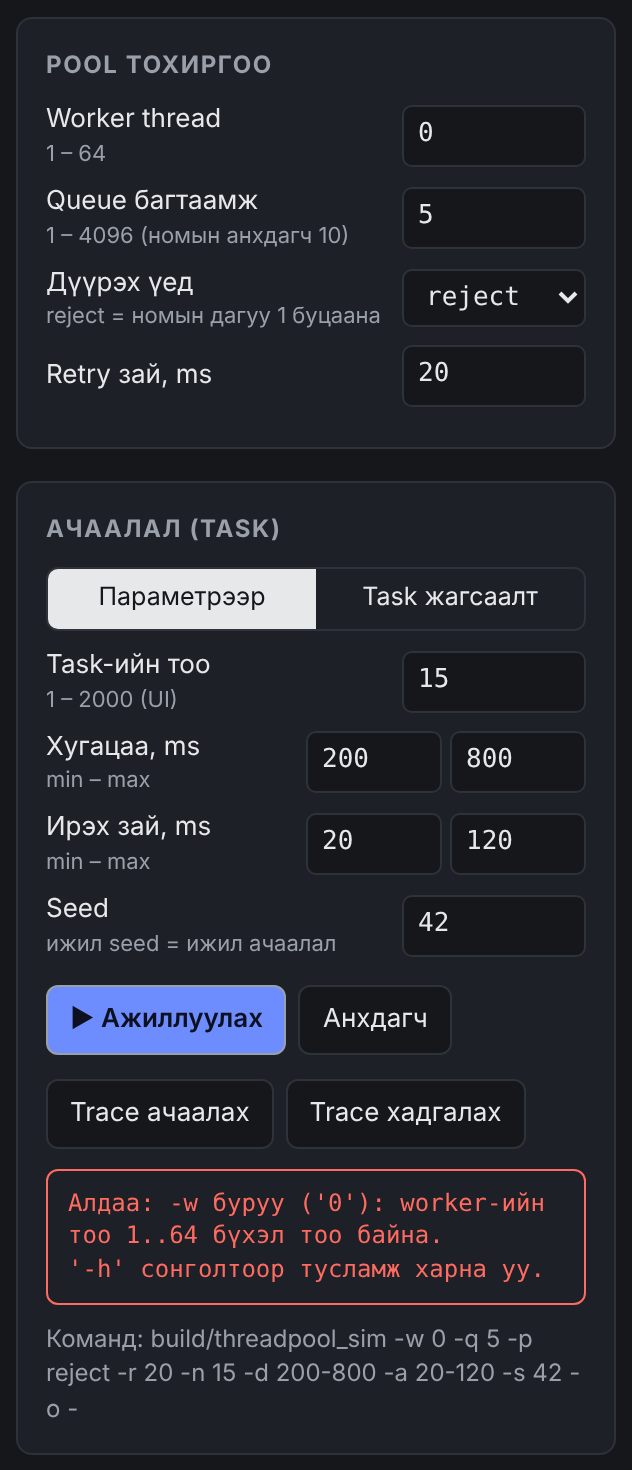
\includegraphics[width=\linewidth]{img/shots/error_workers0.png}}}\end{minipage}\hspace{4mm}\begin{minipage}[t]{0.346\linewidth}\vspace{0pt}{\setlength{\fboxsep}{0pt}\setlength{\fboxrule}{0.5pt}\fcolorbox{frameline}{white}{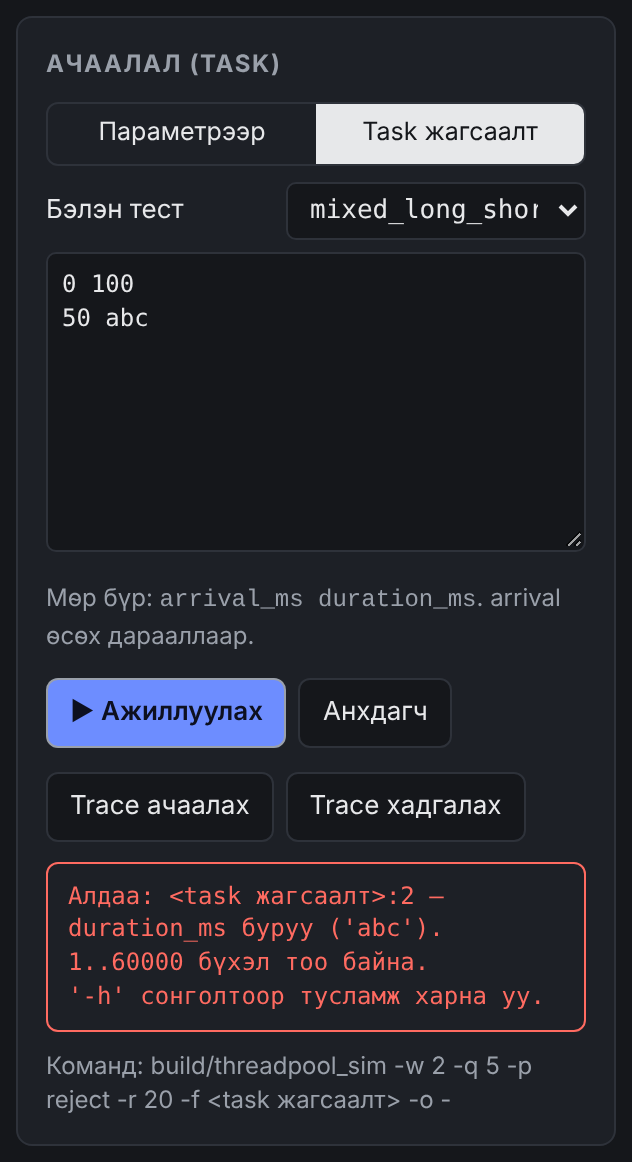
\includegraphics[width=\linewidth]{img/shots/error_file.png}}}\end{minipage}
\caption{Буруу оролт: worker = 0 (зүүн), task жагсаалтад тоо биш утга (баруун)}\label{fig:err}
\end{figure}

% ======================================================================
\section{Operational заавар}

\subsection{Repository clone}

\par\noindent\begin{minipage}{\linewidth}\setlength{\topsep}{1pt}\setlength{\partopsep}{0pt}
\begin{Verbatim}[commandchars=\\\{\}]
git\PY{+w}{ }clone\PY{+w}{ }https://github.com/NominjinNomio/F.CSM302\PYZhy{}BD\PYZus{}IV\PYZhy{}2\PYZhy{}9\PYZhy{}threadpool.git
\PY{n+nb}{cd}\PY{+w}{ }F.CSM302\PYZhy{}BD\PYZus{}IV\PYZhy{}2\PYZhy{}9\PYZhy{}threadpool
git\PY{+w}{ }checkout\PY{+w}{ }v1.0\PY{+w}{      }\PY{c+c1}{\PYZsh{} 9\PYZhy{}р долоо хоногт нийтэлсэн хувилбар}
\end{Verbatim}
\end{minipage}

\subsection{OS, compiler/runtime, version}

\begin{table}[H]
\centering
\caption{Туршсан орчин}\label{tab:env}
\begin{tabular}{|P{0.220}|P{0.320}|P{0.280}|P{0.180}|}
\hline
\rowcolor{tablehead} \textbf{Орчин} & \textbf{OS} & \textbf{Compiler} & \textbf{Python} \\ \hline
Хөгжүүлэлт, тест & Ubuntu 24.04.5 LTS, x86\_64 & gcc 13.3.0 & 3.13.18 \\ \hline
GitHub Actions & ubuntu-latest & gcc & 3 \\ \hline
GitHub Actions & macos-latest & Apple clang & 3 \\ \hline
\end{tabular}
\end{table}

Шаардлага: C11 compiler (gcc ≥ 9 эсвэл clang ≥ 10) + \code{make}, Python 3.8 эсвэл түүнээс дээш, орчин үеийн browser. Python-д pip сан, интерфейст интернет (CDN) шаардлагагүй.

\subsection{Dependency суулгах}

\par\noindent\begin{minipage}{\linewidth}\setlength{\topsep}{1pt}\setlength{\partopsep}{0pt}
\begin{Verbatim}[commandchars=\\\{\}]
\PY{c+c1}{\PYZsh{} Ubuntu / Debian / WSL2}
sudo\PY{+w}{ }apt\PY{+w}{ }update\PY{+w}{ }\PY{o}{\PYZam{}\PYZam{}}\PY{+w}{ }sudo\PY{+w}{ }apt\PY{+w}{ }install\PY{+w}{ }\PYZhy{}y\PY{+w}{ }build\PYZhy{}essential\PY{+w}{ }python3
\PY{c+c1}{\PYZsh{} Fedora}
sudo\PY{+w}{ }dnf\PY{+w}{ }install\PY{+w}{ }\PYZhy{}y\PY{+w}{ }gcc\PY{+w}{ }make\PY{+w}{ }python3
\PY{c+c1}{\PYZsh{} macOS}
xcode\PYZhy{}select\PY{+w}{ }\PYZhy{}\PYZhy{}install
\end{Verbatim}
\end{minipage}

\subsection{Build ба Run}

\par\noindent\begin{minipage}{\linewidth}\setlength{\topsep}{1pt}\setlength{\partopsep}{0pt}
\begin{Verbatim}[commandchars=\\\{\}]
make\PY{+w}{                         }\PY{c+c1}{\PYZsh{} build/threadpool\PYZus{}sim, build/client}
make\PY{+w}{ }ui\PY{+w}{                      }\PY{c+c1}{\PYZsh{} UI сервер, http://localhost:8000}
make\PY{+w}{ }client\PY{+w}{                  }\PY{c+c1}{\PYZsh{} номын client.c жишээ}
make\PY{+w}{ }run\PY{+w}{                     }\PY{c+c1}{\PYZsh{} жишээ run \PYZhy{}\PYZgt{} build/trace.json}
\PY{c+c1}{\PYZsh{} core\PYZhy{}ийг шууд ажиллуулах:}
./build/threadpool\PYZus{}sim\PY{+w}{ }\PYZhy{}w\PY{+w}{ }\PY{l+m}{3}\PY{+w}{ }\PYZhy{}q\PY{+w}{ }\PY{l+m}{5}\PY{+w}{ }\PYZhy{}n\PY{+w}{ }\PY{l+m}{15}\PY{+w}{ }\PYZhy{}d\PY{+w}{ }\PY{l+m}{200}\PYZhy{}800\PY{+w}{ }\PYZhy{}a\PY{+w}{ }\PY{l+m}{20}\PYZhy{}120\PY{+w}{ }\PYZhy{}o\PY{+w}{ }trace.json
./build/threadpool\PYZus{}sim\PY{+w}{ }\PYZhy{}w\PY{+w}{ }\PY{l+m}{2}\PY{+w}{ }\PYZhy{}q\PY{+w}{ }\PY{l+m}{3}\PY{+w}{ }\PYZhy{}f\PY{+w}{ }tests/burst.txt\PY{+w}{ }\PYZhy{}p\PY{+w}{ }retry
./build/threadpool\PYZus{}sim\PY{+w}{ }\PYZhy{}h\PY{+w}{    }\PY{c+c1}{\PYZsh{} бүх сонголт}
\end{Verbatim}
\end{minipage}

Exit код: \textbf{0} амжилттай, \textbf{2} буруу оролт, \textbf{3} ажиллах үеийн алдаа (санах ой, thread үүсгэх), \textbf{4} дотоод шалгалт унасан.

\subsection{Үндсэн тестийн өгөгдөл}

\par\noindent\begin{minipage}{\linewidth}\setlength{\topsep}{1pt}\setlength{\partopsep}{0pt}
\begin{Verbatim}[commandchars=\\\{\}]
make\PY{+w}{ }\PY{n+nb}{test}
\end{Verbatim}
\end{minipage}

\begin{itemize}
  \item \code{./build/client}: номын жишээ, 5 хос тооны нийлбэр (15, 3, 300, 0, 42).
  \item \code{tests/basic.txt}: 10 task, W=3, Q=10 → хүлээн авсан 10, татгалзсан 0, зэрэг ≤ 3.
  \item \code{tests/burst.txt}: 10 × 300 мс, t=0; W=2, Q=3 → reject үед 3-5 хүлээн авна, retry үед 10.
  \item \code{tests/fifo.txt}: 6 task, W=1 → START дараалал T0…T5.
  \item \code{tests/mixed\_long\_short.txt}: 1 × 1500 мс + 7 × 100 мс, W=3.
\end{itemize}

Trace-ийг бие даан шалгах: \code{python3 tests/verify\_trace.py trace.json --expect accepted=15}.

\subsection{Нэмэлт boundary ба error тест}

\par\noindent\begin{minipage}{\linewidth}\setlength{\topsep}{1pt}\setlength{\partopsep}{0pt}
\begin{Verbatim}[commandchars=\\\{\}]
\PY{c+c1}{\PYZsh{} queue 1: татгалзал гарна}
./build/threadpool\PYZus{}sim\PY{+w}{ }\PYZhy{}w\PY{+w}{ }\PY{l+m}{1}\PY{+w}{ }\PYZhy{}q\PY{+w}{ }\PY{l+m}{1}\PY{+w}{ }\PYZhy{}n\PY{+w}{ }\PY{l+m}{6}\PY{+w}{ }\PYZhy{}d\PY{+w}{ }\PY{l+m}{100}\PY{+w}{ }\PYZhy{}a\PY{+w}{ }\PY{l+m}{0}
\PY{c+c1}{\PYZsh{} дээд 64 worker}
./build/threadpool\PYZus{}sim\PY{+w}{ }\PYZhy{}w\PY{+w}{ }\PY{l+m}{64}\PY{+w}{ }\PYZhy{}q\PY{+w}{ }\PY{l+m}{64}\PY{+w}{ }\PYZhy{}n\PY{+w}{ }\PY{l+m}{64}\PY{+w}{ }\PYZhy{}d\PY{+w}{ }\PY{l+m}{50}\PY{+w}{ }\PYZhy{}a\PY{+w}{ }\PY{l+m}{0}
\PY{c+c1}{\PYZsh{} 500 task stress}
./build/threadpool\PYZus{}sim\PY{+w}{ }\PYZhy{}w\PY{+w}{ }\PY{l+m}{8}\PY{+w}{ }\PYZhy{}q\PY{+w}{ }\PY{l+m}{16}\PY{+w}{ }\PYZhy{}n\PY{+w}{ }\PY{l+m}{500}\PY{+w}{ }\PYZhy{}d\PY{+w}{ }\PY{l+m}{1}\PYZhy{}3\PY{+w}{ }\PYZhy{}a\PY{+w}{ }\PY{l+m}{0}\PY{+w}{ }\PYZhy{}p\PY{+w}{ }retry\PY{+w}{ }\PYZhy{}r\PY{+w}{ }\PY{l+m}{1}
make\PY{+w}{ }tsan\PY{+w}{     }\PY{c+c1}{\PYZsh{} ThreadSanitizer}
\end{Verbatim}
\end{minipage}

\begin{longtable}{|P{0.240}|P{0.760}|}
\caption{Буруу оролтын тестийн бодит гаралт (exit 2)}\label{tab:errout}\\
\hline
\rowcolor{tablehead} \textbf{Тест} & \textbf{Программын мэдээлэл} \\ \hline
\endfirsthead
\hline
\rowcolor{tablehead} \textbf{Тест} & \textbf{Программын мэдээлэл} \\ \hline
\endhead
\code{err\_workers\_0} & Алдаа: -w буруу ('0'): worker-ийн тоо 1..64 бүхэл тоо байна. \\ \hline
\code{err\_workers\_65} & Алдаа: -w буруу ('65'): worker-ийн тоо 1..64 бүхэл тоо байна. \\ \hline
\code{err\_queue\_0} & Алдаа: -q буруу ('0'): queue-ийн багтаамж 1..4096 байна. \\ \hline
\code{err\_queue\_text} & Алдаа: -q буруу ('abc'): queue-ийн багтаамж 1..4096 байна. \\ \hline
\code{err\_tasks\_0} & Алдаа: -n буруу ('0'): task-ийн тоо 1..10000 байна. \\ \hline
\code{err\_dur\_0} & Алдаа: -d буруу ('0'): 'MIN' эсвэл 'MIN-MAX', 1..60000 ms. \\ \hline
\code{err\_dur\_order} & Алдаа: -d буруу ('500-100'): MIN нь MAX-аас их байж болохгүй. \\ \hline
\code{err\_gap\_neg} & Алдаа: -a буруу ('-5'): 'MIN' эсвэл 'MIN-MAX', 0..60000 ms. \\ \hline
\code{err\_policy} & Алдаа: -p буруу ('fifo'): 'reject' эсвэл 'retry' байна. \\ \hline
\code{err\_missing\_val} & Алдаа: '-w' сонголтод утга өгөөгүй байна. \\ \hline
\code{err\_unknown\_opt} & Алдаа: Танигдаагүй сонголт '-x'. \\ \hline
\code{err\_file\_missing} & Алдаа: 'tests/no\_such\_file.txt' файлыг нээж чадсангүй (No such file or directory). \\ \hline
\code{err\_file\_number} & Алдаа: tests/bad\_number.txt:2 — arrival\_ms буруу ('abc'). 0..3600000 бүхэл тоо байна. \\ \hline
\code{err\_file\_sorted} & Алдаа: tests/bad\_unsorted.txt:2 — arrival\_ms өсөхгүй дарааллаар байна ('50'). Эрэмбэлэгдсэн байх ёстой. \\ \hline
\code{err\_file\_columns} & Алдаа: tests/bad\_columns.txt:1 — мөр бүр 'arrival\_ms duration\_ms' гэсэн 2 тоотой байх ёстой. \\ \hline
\code{err\_file\_dur0} & Алдаа: tests/bad\_duration.txt:1 — duration\_ms буруу ('0'). 1..60000 бүхэл тоо байна. \\ \hline
\code{err\_file\_empty} & Алдаа: 'tests/bad\_empty.txt' файлд нэг ч task алга. \\ \hline
\end{longtable}

\subsection{Хүлээгдсэн үр дүн}

\begin{itemize}
  \item \code{make test}: төгсгөлд \code{Нийт: 29 PASS, 0 FAIL}, exit 0.
  \item Ажиллуулалт бүрийн stderr-ийн төгсгөлд 8 мөр \code{[ OK ]} ба \code{VERIFY: OK}.
  \item \code{make tsan}: ThreadSanitizer-ийн \code{WARNING} гарахгүй, \code{VERIFY: OK}.
  \item Хугацааны утгууд (хүлээлт, makespan) машин бүрт хэдэн мс-ээр зөрнө; хүлээн авсан/татгалзсан тоо, FIFO, зэрэгцээний дээд хэмжээ өөрчлөгдөхгүй (burst-ийн 3-5 мужаас бусад).
  \item GitHub Actions: build-and-test (linux, macos) ногоон.
\end{itemize}

\subsection{Known issues}

\begin{itemize}
  \item macOS нэргүй POSIX semaphore (\code{sem\_init}) дэмждэггүй тул \code{dispatch\_semaphore} ашиглана; macOS-ийг зөвхөн CI-д шалгасан.
  \item Windows дээр шууд ажиллахгүй; WSL2 эсвэл VM ашиглана.
  \item Worker-ийн хуваарилалт ба burst үеийн хүлээн авах тоо ажиллуулалт бүрт бага зэрэг өөр (OS scheduler).
  \item Интерфейсээр нэг ажиллуулалт ≤ 2000 task, ≈ 60 с. Илүүг CLI-ээр ажиллуулж, trace-ийг ачаалж үзнэ (их task-тай trace зурахад browser удааширч болно).
  \item Retry горимд нэг client thread хүлээдэг тул дараагийн task-уудын ирэлт хойшилно.
  \item Маш богино (< 1 мс) task-д trace-ийн mutex хэмжилтэд нөлөөлнө.
\end{itemize}

\end{document}
